\documentclass[thesis.tex]{subfiles}

\begin{document}

\chapter{Design}\label{chap:design}

\section{Erarbeitung aller Funktionen}\label{chap:funktionen}
Nach Auswertung der Anforderungen lassen sich folgende Funktionen herausarbeiten, die der LW-Modus können muss.

(voralarme können ja über display weggedrückt werden im kaptiel funktion ergänzen?)

\begin{itemize}
    \item Verbindungsaufbau und Verbindungsabbau sowie Wiederherstellung einer verlorenen Verbindung
    \item Alarmierung des Alleinarbeiters und des Überwachungszentrums
    \item Abrufen von Echtzeit Audio- und Videostreams
    \item Zweiwege Sprachkommunikation
    \item Positionsübermittlung zur Standortüberwachung und für Geofencing
    \item Übermittlung von Textnachrichten
\end{itemize}

Die Grundfunktionalität des LW-Modus ist die Sicherstellung einer ununterbrochenen Verbindung zwischen dem Alleinarbeiter und einem Überwachungszentrum über die Body-Cam.
Um das sicherzustellen, wird ein sauberer Verbindungsaufbau und -abbau beim Einschalten oder Ausschalten der Body-Cam nötig.
Um nach Aktivierung des LW-Modus eine durchgängige Verbindung zu gewährleisten, muss das Programm einen Verbindungsverlust innerhalb weniger Sekunden feststellen.
Danach soll automatisch mit dem Wiederaufbau der Verbindung fortgefahren werden.
Hierzu verbindet sich die Body-Cam nach einschalten mit einer vorher eingestellten URL, dem Überwachungszentrum.
Beim Anmelden übermittelt sie wichtige Informationen, wie Identifikationsnummer und Standort.
Außerdem Parameter, wie die Dauer nach dem bei Verbindungsverlust ein Alarm ausgelöst wird.
Diese Verbindung dient vorerst der Anmeldung und Positionsübermittlung ohne ununterbrochene Verbindungsüberwachung und kann jederzeit vom Alleinarbeiter beendet werden.
Beim Beenden der Verbindung wird diese sauber abgebaut und die Body-Cam meldet sich beim Überwachungszentrum ab.
Wenn ein Verbindungsverlust eintritt, wird eine automatische Wiederherstellung ohne Alarmauslösung ausgeführt.
Bei eingeschalteten LW-Modus geht die Verbindung in einen strengeren Zustand über.
In diesem wird ein Verbindungsverlust unmittelbar festgestellt und geht auf beiden Seiten mit Auslösung eines Alarms einher, falls die Verbindung in einer vorher definierten Zeit nicht wiederhergestellt werden kann.
\\

Die Alarmierung besteht aus einer Alarmmeldung, die auf beiden Seiten der Verbindung dargestellt wird.
Sie kann visuell, akustisch und haptisch sein.
Die Meldung soll dazu dienen den Träger der Body-Cam sowie einen Operator in einem Überwachungszentrum über ein bestimmtes Ereignis zu informieren und die Aufmerksamkeit auf dieses zu lenken.
Diese können von einfachen aber wichtigen Informationen wie Akkustand oder das Verlassen oder Betreten eines bestimmten Bereiches, über kritische Meldungen wie Gefahrensituationen oder eine längere unterbrochene Verbindung gehen.
So kann der LW den Alarm beispielsweise durch ein lautes Piepen ähnlich einem Feuermelder, durch Vibration der Body-Cam, durch schnell blinkende LEDs bzw. des Displays oder einer Mischung aus diesen Szenarien mitbekommen.
Das hat den Vorteil, dass der Träger in jeder Situation optimal informiert werden kann.
Die Vibration des Gerätes kann als stiller Alarm genutzt werden.
So wird der LW auf eine bestimmte Situation aufmerksam gemacht, ohne die Aufmerksamkeit der Umgebung auf ihn zu lenken.
Für das Überwachungszentrum spielen diese unterschiedlichen Möglichkeiten keine tragende Rolle.
Hier kommen nur visuelle und akustische Meldungen zum Einsatz, die einen möglichen Operator über eine Situation alarmieren sollen.
Die Priorität der Alarmmeldungen kann durch die unterschiedlichen Möglichkeiten und deren Intensität gesteuert werden.
Zum Beispiel bekommt der LW und das Überwachungszentrum eine kurze Meldung auf dem Display bzw. Monitor begleitet von einem kurzen Piepton, wenn der Akkustand des Geräts unter 25 Prozent fällt.
Dies zählt damit zu den unwichtigeren Meldungen und soll die Beteiligten nur für bevorstehende Ereignisse sensibilisieren.
Die Intensität dieser Meldung steigt, wenn der Akkustand einen kritischen Punkt erreicht.
Hierzu könnten dann lautere und längere Pieptöne sowie Vibration der Body-Cam genutzt werden.
Wenn ein akuter Gefahrenfall auftritt, sollte sich die Alarmmeldung signifikant von anderen unterscheiden, um damit die volle Aufmerksamkeit des LW und des Überwachungszentrums auf die Situation zu lenken.
\\

Der Abruf von Echtzeit Audio- und Videostreams soll ebenfalls von der Body-Cam umgesetzt werden.
Eine Video- und Audioaufzeichnung sowie die Möglichkeit diese zu streamen bietet die Body-Cam bereits, wie in \autoref{chap:grundlagen} beschrieben.
Diese Option soll auch für den LW-Modus zur Verfügung stehen.
Dabei kann ein Operator eine Anfrage an eine Body-Cam stellen, um die jeweiligen Streams vom Gerät abzurufen und im Überwachungszentrum anzeigen zu lassen.
Diese Möglichkeit kann vor allem im Bereich einer Mobilfunkverbindung nur eingeschränkt nutzbar sein.
So müssen hier aufgrund von Verbindungsstärke und -qualität Einbußen bei Verfügbarkeit und Qualität der Streams gemacht werden.
Bei einer guten WLAN-Abdeckung, wie sie in Gebäuden eingesetzt werden kann, besteht dieses Problem weniger.
Hier kann durch die Nutzung einer WLAN-Verbindung eine wesentliche höhere Bandbreite und Verbindungsstärke genutzt werden.
Außerdem haben Unternehmen die Möglichkeit die Abdeckung ihrer WLAN-Verbindung auszubauen, um eine bessere Qualität der Verbindung zu gewährleisten.
Diese Option besteht bei der Nutzung der öffentlichen Mobilfunknetze nicht.
\\

Neben einer aktiven Anfrage durch das Überwachungszentrum kann der Stream bei Bedarf auch im Alarmfall übertragen werden.
Hierfür kann die Body-Cam automatisch die Streams an das Zentrum übertragen, wenn der LW einen Alarm auslöst.
Dies hat den Vorteil das der Operator nach Eingang einer Alarmmeldung sofort die Möglichkeit hat sich ein Bild von dem Gefahrenfall zu machen.
Er kann dafür die Informationen aus Bild und Ton nutzen, um die Situation besser einzuschätzen und bei Bedarf weitere Schritte einzuleiten.
\\

Um den Informationsaustausch weiter zu verbessern, baut die Body-Cam nach Bedarf einen Zweiwege-Sprachkanal zwischen dem Operator und dem LW auf.
Dieser ermöglicht einen aktiven Austausch zwischen Träger und Empfangseinrichtung.
Der Austausch von Informationen findet damit nicht mehr nur einseitig in Richtung des MC statt.
So hat der LW die Möglichkeit sich mit einem Mitarbeiter in der Empfangseinrichtung über verschiedene Situation auszutauschen.
Das trägt unter anderem zur Minderung des Isolationsgefühls(Quelle wie in Einleitung?) bei.
Außerdem kann ein Operator beispielsweise, nach dem er in einer Gefahrensituation bereits Informationen durch die Streams erhalten hat, den LW kontaktieren, um weitere Sachverhalte zu bekommen und mehr Klarheit über die Situation zu gewinnen.
\\

Eine weitere Funktion ist die Standortübermittlung.
Die Body-Cam übermittelt kontinuierlich ihren Standort an das Überwachungszentrum.
Die Genauigkeit der Position wird durch die Verbindung von GPS, Mobilfunk, WLAN und Bluetooth erhöht.
Dies ist in erster Linie wichtig um bei einem Notfall den exakten Standort der in Gefahr befindlichen Person zu detektieren.
So können Notfallkräfte im Ernstfall schnell und gezielt reagieren.
Ein weiterer Vorteil dieser Positionsüberwachung ist das sogenannte "Geofencing".
Dies beschreibt das automatische Auslösen bestimmter Aktion beim Ein- oder Austritt aus einem vorher festgelegten Bereich.
(https://de.wikipedia.org/wiki/Geofencing finde noch keine bessere Quelle).
In Bezug auf den LW-Modus könnten diese Aktionen z.B. das Ein- oder Ausschalten des Modus sein, wenn der Träger mit seiner Schicht beginnt und den zu überwachenden Bereich betritt.
Außerdem wäre es möglich einen Bereich mit besonders hohen Gefahrenpotenzial zu markieren.
Der LW würde dann bei betreten über diesen Umstand per Body-Cam informiert werden, damit er die volle Konzentration auf seine Sicherheit lenken kann.
Zusätzlich kann die Standortüberwachung in die Protokollierung der Alleinarbeit mit einfließen um diese mit Informationen über Laufwege und Aufenthaltsdauer zu verbessern.
\\

\begin{figure}[h]
    \centering
    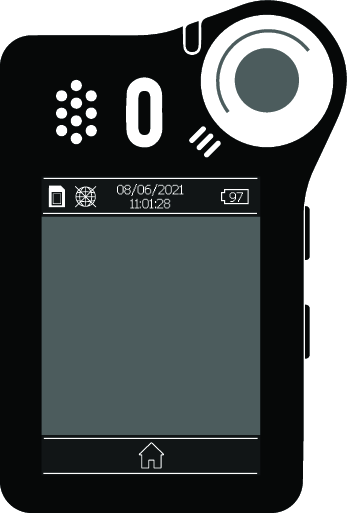
\includegraphics[height=0.4\textwidth]{/BC_schema_front.png}
    \caption{Schemata der Front einer Body-Cam}
    \label{fig:BC_schema}
\end{figure}

Durch das vorhandene Display mit Touch-Funktion besteht die Möglichkeit zum anzeigen und beantworten von Textnachrichten.
Mit den Nachrichten kann das Überwachungszentrum dem LW kurze Informationen übermitteln oder nach dem Status fragen, ohne eine Sprachverbindung zu benutzen.
Die Beantwortung kann der Träger über vorher definierte Antworten übernehmen, die als Buttons auf dem Display erscheinen.
Automatisch generierte Textnachrichten können zur Unterstützung genutzt werden.
Sie können nach bestimmten Ereignissen mehr Informationen bereitstellen.
Unter diese Events zählen beispielsweise Alarmauslösung, Ein- oder Austritt aus einem Geofencing-Bereich, Fehlfunktionen oder Statusveränderungen der Body-Cam.
Außerdem wird das Display dafür genutzt, alle möglichen Statusinformationen über das Gerät anzuzeigen, wie Akkustand, Mobilfunkstärke oder Temperatur.
\\

\section{Protokolldesign}\label{chap:protokolldesign}
Damit alle Anforderungen an die Kommunikation zwischen BC und MC erfüllt werden können, wird ein eigenes Protokoll verwendet.
%%
Dieses wird in der einheitlichen und weit verbreiteten „JavaScript Object Notation“ (JSON) verfasst.
%%
Dieser Standard hat für die Anwendung folgende Vorteile.
%%
Das Protokoll kann einfach zwischen Client und Server übertragen werden, da JSON sehr einfach in einen String umgewandelt werden kann.
%%
Es existieren bereits in sehr vielen Programmiersprachen Bibliotheken die JSON verstehen, bearbeiten und umwandeln können,
welche Nachrichten schnell zwischen verschiedenen Anwendungen konvertiert werden können, wenn dies benötigt wird.
%%
Das Protokoll kann durch diese Form einfach und schnell erweitert oder angepasst werden.
%%
Durch seine einheitliche Struktur und Hierarchieebenen wird dieser Effekt verstärkt und die Nachrichten können dadurch gut strukturiert werden.
%%
Es ist menschenlesbar und kann somit ohne spezielles Programm von Menschen gelesen und verstanden werden.
%%
Dies hilft z.B. beim Debuggen oder um Protokolleinträge schneller lesen zu können.
%%
\\

Das entwickelte Protokoll enthält folgende Informationen: Zeitstempel, Referenznummer, Nachrichtentyp, Nachrichteninhalt, Antwortreferenznummer.
%%
Der Zeitstempel wird der Nachricht beim Erstellen gegeben, damit der zeitliche Verlauf nachvollzogen werden kann und die
Nachrichten in einem Verlaufsprotokoll angelegt werden können.
%%
Die Referenznummer wird aufsteigend für jede Nachricht vergeben und macht diese eindeutig identifizierbar.
%%
Diese Nummer wird auch als Referenznummer für eine Antwort auf eine bestimmte Nachricht genutzt.
%%
Diese wird dann unter Antwortreferenznummer der Nachricht mitgeben und findet nur bei Nachrichten des Typs „Antwort“ Anwendung.
%%
Der Nachrichtentyp gibt an, welchen Typ die geschickte Mitteilung hat.
%%
Hier gibt es momentan die Typen Anfrage, Antwort, Herzschlag und initiale Nachricht.
%%
Herzschlag wird immer dann vergeben, wenn ein Nachrichtenaustausch zwischen Client und Server stattfindet, der zur Verbindungssicherung dient.
%%
Die initiale Nachricht schickt der Client einmalig am Anfang einer Verbindung an dem Server,
um ihm Einstellungs- und Verbindungsparameter mitzuteilen.
%%
Im Nachrichteninhalt befindet sich alles, was die Mitteilung als Daten beinhaltet.
%%
Dies können beispielsweise gerade genannte Parameter oder Anfrage bzw. Antwortdetails sein.
%%
Durch den Aufbau der JSON kann das Datenfeld bei Bedarf ebenfalls strukturiert werden, um auch größere Datenmengen gut abbilden zu können.
%%
\\

(TODO: Quellen für Vorteile bzw. zum Aufbau von JSON finden)

\section{Primitiven}\label{chap:primitiven}
Im folgenden Kapitel werden alle Primitiven aufgeführt und beschrieben.
%%
Das sind alle Informationen, die der LW-Modus von der BC braucht, um die vollständige Funktion zu gewährleisten
und um alle Anfragen des MC zu beantworten.
%%
\\

Um die Grundfunktionalität des Geräts und damit der Funktion des LW-Modus sicher zu stellen, werden in erster Linie
die Vitalwerte des Geräts benötigt.
%%
Zudem alle weiteren Informationen, die es über die BC gibt.
%%
Darunter zählen die eindeutige Identifikationsnummer, die aktuelle Versionsnummer der Firm- und Software,
ein aktueller Zeitstempel, der Batteriestatus, der vorhandene Speicherplatz für Bild- und Videodateien,
die Temperatur Innen und Außen \textcolor{red}{(nochmal nachfragen)}, die Mobilfunkstärke sowie Informationen über die Mobilfunkverbindung,
wenn das Gerät ins Netz eingewählt ist, WLAN-Stärke und Verbindungsdetails, falls eine WLAN-Verbindung besteht und
der letzte bekannte Standort der BC.
%%
\\

Informationen, die sich schnell ändern können, wie Verbindungsdetails und -stärken, der letzte Standort und
einen aktuellen Zeitstempel soll die BC alle 1-5 Sekunden bereitstellen können.
%%
Batteriestatus, Temperatur und Speicherplatz die zum Überwachen des Gerätezustands wichtig sind, sollten alle 30 Sekunden aktualisiert werden.
%%
Einmalig zum Start der Software werden Versions- und Identifikationsnummern benötigt.
%%
Da diese Angaben sich während des Betriebs nicht ändern können.
%%
\\

Damit die BC dem LW während aktiven Lone-Workers-Modus einen Alarmfall mitteilen kann,
muss es die Möglichkeit geben die Lautsprecher, den Vibrationsmechanismus sowie die LEDs ansteuern zu können.
%%
Dies wird benötigt um akustische, haptische und visuelle Alarmmeldungen an den LW weiter zu reichen.
%%
Der Lautsprecher wird neben dem Abspielen von Alarmtönen noch für das Abspielen von Audionachrichten verwendet.
%%
Außerdem soll es möglich seine Informationen auf dem Display anzuzeigen.
%%
Dies findet Anwendung für Textnachrichten vom MC oder Alarmursachen.
%%
Bei letzterem kann der LW nach einem Alarm mehr Informationen über die Art der Warnung bekommen.
%%
Beispielsweise ob und welcher Gerätefehler vorliegt oder wie lange eine Mobilfunkverbindung schon getrennt ist.
%%
\\

Der LW-Modus muss die Möglichkeit haben den Video- und Audiostream der BC zu aktivieren.
%%
Auf Anfrage des MC soll die BC die beiden Streams über eine gesicherte Verbindung dem MC zur Verfügung stellen,
damit das Center den LW bei Bedarf live überwachen kann.
%%
Außerdem soll dies nach selbem Schema auch für den Two-Way-Audio Kanal vollzogen werden.
%%
Dies dient dazu, eine aktive Sprachverbindung zwischen MC und LW zu realisieren, damit im Gefahrenfall schnell reagiert
und Informationen ausgetauscht werden können.
%%

\section{Beschreibung der Statusmaschinen}


\subfilebib % Makes bibliography available when compiling as subfile
\end{document}